\paragraph {}
Ahora que ya sabemos calcular la ganancia del SiPM a partir de una toma de datos procedemos a determinar la dependencia que presenta el SiPM con la temperatura. En concreto nos interesa determinar el comportamiento de su ganancia cuando varía la temperatura. Para ello realizaremos una serie de medidas a distintas temperaturas y, para cada una de ellas, calcularemos la ganancia a partir del metodo expuesto en el punto anterior.

\paragraph {}
Nos centraremos en el rango de temperatura entre 15 grados, que es el mínimo que nos permitía llegar el sistema de control de temperatura y 41 grados, que, suponemos, será el límite al que llegará nuestro futuro detector en la práctica. Es decir, este rango de temperaturas será equivalente a las temperaturas a las que estará sometido nuestro detector debido a las condiciones climáticas del lugar. Realizaremos pasos de 2 grados entre cada medida realizando un total de 14 medidas. Únicamente realizaremos medidas de 15000 eventos ya que son más que suficiente para obtener un espectro suficientemente suave. 

\paragraph {}
Para automatizar este proceso procedemos a desarrollar una macro en ROOT que realice este ajuste. Esta macro se divide en dos partes:
\begin{itemize}
\item{} Por un lado posee un bucle en el que, en cada paso, abre el fichero correspondiente a una temperatura, empezando por la mínima (15 grados) realiza todo el estudio anterior y guarda ganancia y temperatura con sus errores en 4 vectores respectivamente. En cada paso aumenta 2 grados la temperatura y pasa a leer el siguiente fichero.

\paragraph {}
Hay que tener en cuenta que, como se dijo anteriormente, el sistema de control de temperatura debe de estar en la zona uno del diagrama de fases existente en la ficha técnica. Esto implico que, para medidas inferiores a 27 grados necesitamos aumentar la humedad en un 5\% a cada medida (humedad del 45\% para 25 grados, 50\% para 23 grados, etc.). Esto no tiene mayor importancia ya que se vio que la ganancia del SiPM no se ve afectada de forma apreciable ante modificaciones de la humedad de este tamaño.

\paragraph {}
La incertidumbre en la temperatura viene dada por la oscilación en el valor de la temperatura observada directamente en el panel de control del sistema. La oscilación observada fue en todo momento de 0.1 grados, una incertidumbre totalmente inapreciable tanto a nivel visual en la gráfica como a nivel de variación de la ganancia.

\item {} Por otro lado, partiendo de estos 4 vectores de dimensión 14 en nuestro caso (igual al número de ficheros que ha leido) que contienen ganancia, temperatura y sus errores de forma ordenada la macro realiza un ajuste lineal. El ajuste obtenido se presenta en la imagen diecinueve.

\begin{figure}[hbtp]
\centering
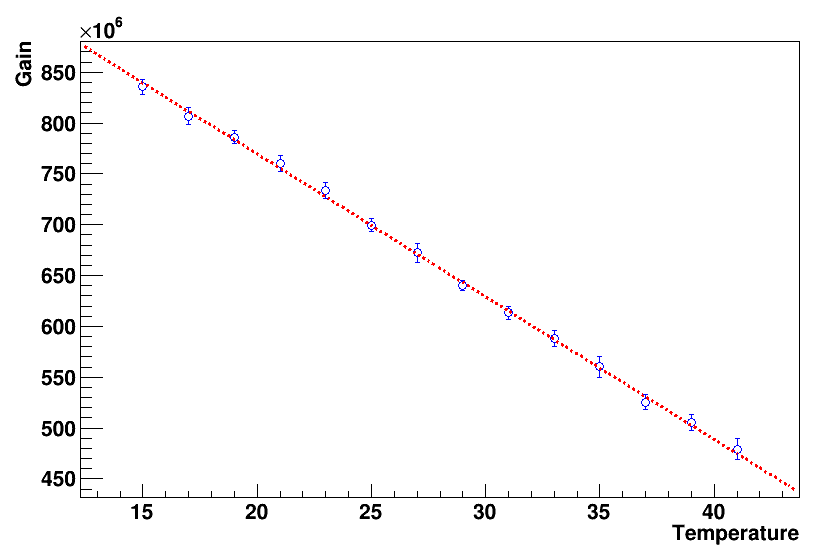
\includegraphics[scale=0.2]{/home/marcos/Documentos/Trabajo_final_de_Master/Trabajo/Figuras/Dependenciatemperatura.png}
\caption{\textbf{Imagen 19}.- Ganancia frente a temperatura}
\end{figure}

Podemos observar la existencia de un comportamiento lineal casi perfecto en un rango de temperatura de 26 grados. Esta es una propiedad que caracteriza al SiPM, una muy buena linealidad en su comportamiento frente a modificaciones en varias magnitudes.

\paragraph {}
Podemos observar que la existencia de un decrecimiento del valor de la ganancia del SiPM a medida que aumenta la temperatura. Esto es debido a que la zona de desertización, que se crea al aplicar un voltaje, y que actuará como zona útil a la hora de detectar las partículas, depende de la temperatura. Al aumentar la temperatura se incrementa la excitación térmica de los portadores de carga pudiendo, de esta forma, invadir la zona de desertización. Esto provoca una reducción de la misma y, por extensión una disminución de la ganancia.

\paragraph {}
La ecuación obtenida en este ajuste $G=aT+b$ toma los siguientes valores: 
\begin{itemize}
\item{} $a=-1.40308 \cdot 10^7 \pm 2.71545 \cdot 10^5$ $T^{-1}$
\item{} $b=1.05001 \cdot 10^9 \pm 7.69711 \cdot 10^6$ $T^{-1}$
\end{itemize}

Esta es un resultado importante, no por el valor numérico, sino porque será la base que utilizaremos para conseguir la compensación de la ganancia.
\end{itemize}